\newpage
\subsection{Spectroscopy}

In this module we study a few of the basic MR signals that can be measured with one or two RF pulses and no gradients. \textbf{Use a water-only phantom for this module}.

\subsubsection{Free Induction Decay} \label{sec:fid}

The most basic MR signal is the Free Induction Decay (FID). An FID results from the action of a single RF pulse, presenting as a damped oscillation of the excited transverse magnetization (Figure \ref{fig:FID}). 

\vspace{5mm}

\noindent{}\color{red}
What is the oscillation frequency for the FID? What mechanism(s) are responsible for damping this oscillation?
\color{black}
% soln: oscillates at the Larmor frequency, damped by T2* decay (which itself is a combination of T2 decay and dephasing due to off-resonance)

\begin{figure}[h]
    \centering
    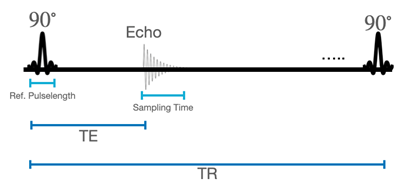
\includegraphics[width=0.7\textwidth]{free-induction-decay}
    \captionsetup{width=.9\textwidth}
    \caption{\label{fig:FID} Pulse sequence inducing free induction decay (FID). A single RF pulse produces a damped oscillation in the transverse magnetization signal.}
\end{figure}

\noindent{Follow these steps to measure an FID signal:} 
\begin{enumerate}
    \item   In the main menu, click \textbf{Spectroscopy} and select the \textbf{Free Induction Decay} sequence.
    \item	Open \textbf{Parameters}. Under \emph{General} set TE to 5 ms, Sampling Time to 6 ms.
    \item	Click \textbf{Acquire}, then \textbf{Data Process}. 

Observe the resulting figures. These plots depict the FID signal in time and frequency domain after demodulation by the center frequency. Hence if the center frequency is well-calibrated you should not see much oscillation, only decay.

    \item Try acquiring a few more FIDs at larger echo times TE.

\end{enumerate}

\subsubsection{Spin Echo}

Another basic MR signal is the Spin Echo. You may have already measured a spin echo in a previous module (e.g. for calibration). Nevertheless we review it here for the purpose of comparison with FID. A spin echo results from the action of two RF pulses, separated by a time TE/2 (Figure \ref{fig:spec-spin-echo}). The spin echo occurs at echo time TE.

\vspace{5mm}

\noindent{}\color{red}
What is the oscillation frequency of a spin echo signal? What mechanism(s) are responsible for shaping the envelope of this oscillation?
\color{black}

\begin{figure}[h]
    \centering
    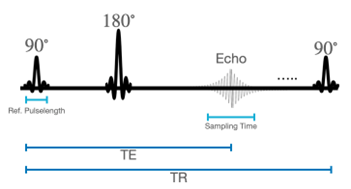
\includegraphics[width=0.7\textwidth]{spin-echo}
    \captionsetup{width=.9\textwidth}
    \caption{\label{fig:spec-spin-echo} Pulse sequence inducing a spin echo at echo time TE. Two RF pulses work to excite then refocus the transverse magnetization signal.}
\end{figure}
\vspace{5mm}

\noindent{Follow these steps to measure a Spin Echo signal:}
\begin{enumerate}
\item	Navigate to the main menu. Click \textbf{Spectroscopy} and select the \textbf{Spin Echo} sequence.
\item	Open \textbf{Parameters}. Under \emph{General} set TE to 10 ms, Sampling Time to 6 ms.
\item	Click \textbf{Acquire}, then \textbf{Data Process}.
\item Try acquiring a few more spin echoes at larger echo times TE.
\end{enumerate}

Observe the resulting figures. As with the FID signal, these plots depict the received signal in time and frequency domains after demodulation by the center frequency, hence the oscillation depicted in Figure \ref{fig:spec-spin-echo} should be largely removed.

\vspace{5mm}

\noindent{}\color{red}
How does the spin echo signal change as you increase TE? Compare with what you observed when you increased TE for the FID signal. Explain the difference.
\color{black}

\vspace{5mm}

\noindent{}\color{red}
Capture screenshots of the resulting plots for both FID and Spin Echo at a few different values of TE.
\color{black}
